\section{A small example}
In this chapter a small Modelica model is compiled, translated and exported to ProMoVis through the export-tool. The files used are available, together with the source code, at GitHub\cite{githabb}\nocite{*}.

\subsection{The input model}

The model used for the example:
\lstset{language=modelica}
\begin{lstlisting}
package QuadTankPack
  model QuadTank
    // Process parameters
	parameter Modelica.SIunits.Area A1=4.9e-4, 
									A2=4.9e-4, 
									A3=4.9e-4, 
									A4=4.9e-4;
	parameter Modelica.SIunits.Area a1(min=1e-6)=0.03e-4, 
									a2=0.03e-4, 
									a3=0.03e-4, 
									a4=0.03e-4;
	parameter Modelica.SIunits.Acceleration g=9.81;
	
	parameter Real 	k1_nmp(unit="m^3/s/V") = 0.56e-6, 
					k2_nmp(unit="m^3/s/V") = 0.56e-6;
	parameter Real g1_nmp=0.30, g2_nmp=0.30;

    // Initial tank levels
	parameter Modelica.SIunits.Length x1_pmv_0 = 0.04102638;
	parameter Modelica.SIunits.Length x2_0 = 0.06607553;
	parameter Modelica.SIunits.Length x3_0 = 0.00393984;
	parameter Modelica.SIunits.Length x4_foo_0 = 0.00556818;
	
    // Tank levels
	Modelica.SIunits.Length x1_pmv(start=x1_pmv_0,min=0.0001);
	Modelica.SIunits.Length x2(start=x2_0,min=0.0001);
	Modelica.SIunits.Length x3(start=x3_0,min=0.0001);
	Modelica.SIunits.Length x4_foo(start=x4_foo_0,min=0.0001);
	Real x1plusx2(start=0);
	// Inputs
	input Modelica.SIunits.Voltage u1;
	input Modelica.SIunits.Voltage u2;

  equation    
    der(x1_pmv) = 	-a1/A1*sqrt(2*g*x1_pmv) + a3/A1*sqrt(2*g*x3) 
					+ g1_nmp*k1_nmp/A1*u1;						
	der(x2) 	= 	-a2/A2*sqrt(2*g*x2) + a4/A2*sqrt(2*g*x4_foo)
					+ g2_nmp*k2_nmp/A2*u2;
	x1plusx2	=	x2+x1_pmv;
	der(x3) 	= 	-a3/A3*sqrt(2*g*x3) 
					+ (1-g2_nmp)*k2_nmp/A3*u2;
	der(x4_foo) = 	-a4/A4*sqrt(2*g*x4_foo) 
					+ (1-g1_nmp)*k1_nmp/A4*u1;

  end QuadTank;
end QuadTankPack;
\end{lstlisting}
This is basically the same model as provided in the JModelica examples with some small changes. The initial values have been configured in such a way that the system is at equilibrium at time zero. As stated earlier, this is something the user has to verify beforehand with the help of the Modelica environment used. Besides the initial values a variable, x1plusx2, have been added to the model. This is done entirely to introduce an algebraic variable in the system.
\subsection{Running the export}
After setup of the input file as depicted in chapter 3, indicating that variables with "\_pmv", "foo\_" and "x2" should be set as measured variables, the exporttool is called. After checking that no warnings were generated, the result can be viewed in ProMoVis:
\setlength\fboxsep{0pt}
\setlength\fboxrule{0.5pt}
\fbox{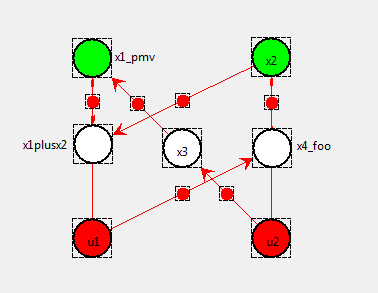
\includegraphics{Figures/exportSFG.png}}\\\newline
As seen,  x1\_pmv and x2 has been set as measured variables, matching with \_pmv and x2 respectively, while none of the variables matched with the pattern "foo\_". If we start by inspecting the process model for x1plusx2:\\\newline
\setlength\fboxsep{0pt}
\setlength\fboxrule{0.5pt}
\fbox{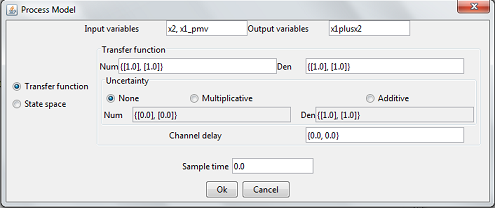
\includegraphics{Figures/x1plusx2Rel.png}}\\\newline
Here, due to the fact that all the variables are represented as Multiple input, single output process models, it doesn't matter which of the incoming arrows to x1plusx2 that is examined. All of the inputs, as depicted in the dialogue, are displayed. As expected, the transfer functions is unity, for both of the input variables to x1plusx2. \\\newline
Examining the properties of the variable yields:

\setlength\fboxsep{0pt}
\setlength\fboxrule{0.5pt}
\fbox{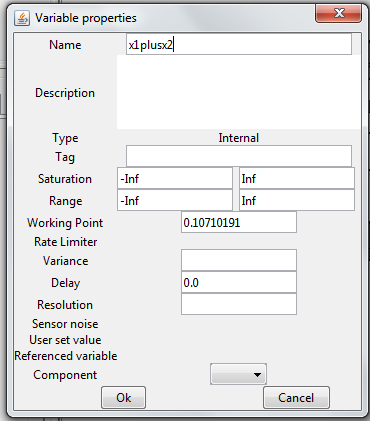
\includegraphics{Figures/x1plusx2OPP.png}}\\\newline
Since the initial values for x1\_pmv and x2 were set in the original model, the working(operating) point of x1plusx2 is the sum of the initial values.\\\newline
Lets look at a variable with some more complex input relations. Choosing x2 it should have both x4\_foo and u2 as inputs and contain a derivative.\\\newline
\setlength\fboxsep{0pt}
\setlength\fboxrule{0.5pt}
\fbox{\includegraphics{Figures/x2rel.png}}\\\newline
From the picture we can see that the input relations are:\\
$\begin{array}{rcl} \frac{-3.4285E-4}{-s -0.05275}*u2 \end{array}$\\
$\begin{array}{rcl} \frac{-0.1817}{-s -0.05275}*x4\_foo \end{array}$\\\newline
Looking at the denominators, they are both the same, recalling the algorithm, described in Appendix \ref{appA}, one can see that this will always be the case for all of the inputs to a variable, they will all share a common denominator.